\documentclass[11pt, addpoints, answers]{exam}

\usepackage{amsmath, amssymb, amsthm, euler}
\usepackage{xcolor}

\usepackage{algorithm}
\usepackage{algorithmicx}
\usepackage{algpseudocode}

\usepackage{tikz}

% headers, footers, titles
\newcommand{\CourseName}{CS101 Algorithms and Data Structures}
\newcommand{\HomeworkNO}{Homework 8}
\newcommand{\DueDate}{Due date: 23:59, November 20th, 2022}

\pagestyle{headandfoot}
\runningheadrule
\runningheader{\CourseName}{\HomeworkNO}{\DueDate}
\runningfooter{}{\thepage}{}

\title{
	\CourseName\\
	Fall 2022\\
	\HomeworkNO
}
\author{}
\date{\DueDate}

% formats of questions, choices, points, etc.
\qformat{\bf\thequestion. (\totalpoints\ points) \thequestiontitle\hfill}
\pointname{'}
\CorrectChoiceEmphasis{\bf\color{blue}}

\newcommand{\fns}{\footnotesize}

\renewcommand{\choiceshook}{
  \setlength{\leftmargin}{25pt}
}

\begin{document}

\maketitle

\begin{enumerate}
  \item Please write your solutions in English.
  \item Submit your solutions to gradescope.com.
  \item Set your FULL name to your Chinese name and your STUDENT ID correctly in Account Settings.
  \item If you want to submit a handwritten version, scan it clearly. \texttt{CamScanner} is recommended.
  \item When submitting, match your solutions to the problems correctly.
  \item No late submission will be accepted.
  \item Violations to any of the above may result in zero points.
\end{enumerate}

\begin{questions}

\titledquestion{Multiple Choices}
Each question has \textbf{one or more} correct answer(s). Select all the correct answer(s). For each question, you will get 0 points if you select one or more wrong answers, but you will get 1 point if you select a non-empty subset of the correct answers.

Write your answers in the following table.

\begin{table}[htbp]
  \centering
  \begin{tabular}{|p{2cm}|p{2cm}|p{2cm}|p{2cm}|}
    \hline
    (a) & (b) & (c) & (d) \\
    \hline
      ABD  &  C   &  C   &   AB  \\
    \hline
  \end{tabular}
\end{table}

\begin{parts}
\part[3] Suppose we use the Prim's algorithm to find the minimum spanning tree of the following graph. Choose all possible sequences of edges added to the minimum spanning tree.
\begin{center}
  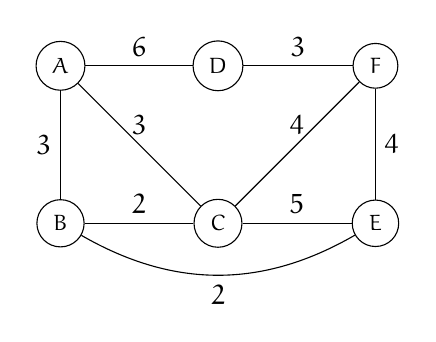
\begin{tikzpicture}[node distance = 2cm]
    \node[draw, circle] (A) {\fns\(A\)};
    \node[draw, circle, below of = A] (B) {\fns\(B\)};
    \foreach \i\j in {B/C, A/D, C/E, D/F} {
      \node[draw, circle, right of = \i] (\j) {\fns\(\j\)};
    }
    \draw[] (A) edge node[left] {\(3\)} (B);
    \foreach \i\j\k in {A/C/3, A/D/6, B/C/2, D/F/3, C/F/4, C/E/5} {
      \draw[] (\i) edge node[above] {\(\k\)} (\j);
    }
    \draw[] (E) edge node[right] {\(4\)} (F);
    \draw[] (B) edge[bend right] node[below] {\(2\)} (E);
  \end{tikzpicture}
\end{center}
\begin{choices}
  \CorrectChoice \(\{A,C\},\{C,B\},\{B,E\},\{C,F\},\{F,D\}\)
  \CorrectChoice \(\{A,B\},\{B,C\},\{B,E\},\{C,F\},\{F,D\}\)
  \choice \(\{A,C\},\{C,B\},\{C,F\},\{B,E\},\{F,D\}\)
  \CorrectChoice \(\{A,B\},\{B,E\},\{B,C\},\{E,F\},\{F,D\}\)
\end{choices}

\part[3] Which of the following statements is/are true?
\begin{choices}
  \choice The time complexity of the Prim's algorithm with a Fibonacci heap is always asymptotically better than that with a binary heap.
  \choice The time complexity of the Prim's algorithm using adjacency list and binary heap is always better than that using adjacency matrix without a priority queue.
  \CorrectChoice The minimum spanning tree of a graph is unique if all the edges have distinct weights.
  \choice The time complexity of the Kruskal's algortihm is \(O\left(|E|\alpha\left(|V|\right)\right)\) if we use the disjoint-sets with union-by-rank optimization and path-compression optimization.
  \choice If \(T\) is a minimum spanning tree obtained by performing the Prim's algorithm starting with vertex \(v\), then for any vertex \(u\) the path on the tree \(T\) connecting \(u\) and \(v\) is the shortest path from \(u\) to \(v\) in the graph.
\end{choices}

\part[3] How many different minimum spanning trees does the following graph have?
\begin{center}
  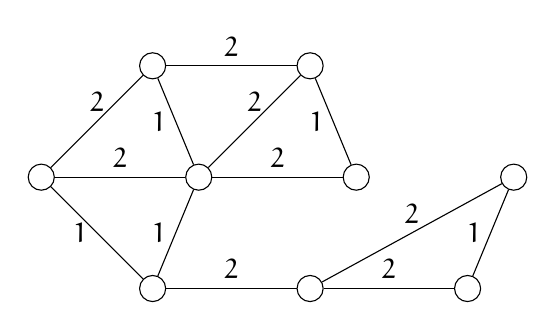
\begin{tikzpicture}[node distance = 2cm]
    \node[draw, circle] (A) {};
    \node[draw, circle, below left of = A] (B) {};
    \node[draw, circle, below right of = B] (D) {};
    \foreach \i\j in {B/C, A/E, C/F, D/G, G/H, F/I} {
      \node[draw, circle, right of = \i] (\j) {};
    }
    \foreach \i\j in {A/E, A/B, C/E, B/C, C/F, D/G, G/H, G/I} {
      \draw[] (\i) edge node[above] {\(2\)} (\j);
    }
    \foreach \i\j in {A/C, E/F, B/D, C/D, H/I} {
      \draw[] (\i) edge node[left] {\(1\)} (\j);
    }
  \end{tikzpicture}
\end{center}
\begin{oneparchoices}
  \choice \(4\)
  \choice \(5\)
  \CorrectChoice \(6\)
  \choice \(7\)
\end{oneparchoices}

\part[3] Suppose \(G=(V,E)\) is an undirected connected graph and that \(T\) is a minimum spanning tree of \(G\). Define \(w(e)\) to be the weight of \(e\) for \(e\in E\). Which of the following statements is/are true?
\begin{choices}
  \CorrectChoice If \(C\subseteq E\) is a cycle in \(G\) and \(e\in C\) is an edge on the cycle such that
  \[\forall f\in C\setminus\{e\},\quad w(e)>w(f),\]
  then \(e\) does not belong to \(T\).
  \CorrectChoice Let \(V=X\cup Y\) be a partition of \(V\) such that \(X\cap Y=\varnothing\). Define
  \[C(X,Y)=\left\{\{u,v\}\in E\mid u\in X,v\in Y\right\}.\]
  If \(e\in C(X,Y)\) is an edge such that
  \[\forall f\in C(X,Y)\setminus\{e\},\quad w(e)<w(f),\]
  then \(e\) must belong to \(T\).
  \choice Suppose \(T^\prime\neq T\) is another minimum spanning tree of \(G\). Let \(w_0\in\left\{w(e)\mid e\in T\right\}\) be the weight of some edge in \(T\). Let \(m\) be the number of edges weighted \(w_0\) in \(T\). Then \(T^\prime\) may contain less than \(m\) edges weighted \(w_0\).
  \choice If \(e\in E\) is an edge that has the largest weight among all edges in \(E\), then \(e\) cannot belong to \(T\).
\end{choices}

\end{parts}

\titledquestion{Minimum Spanning Tree}
Consider the following weighted undirected graph.
\begin{center}
  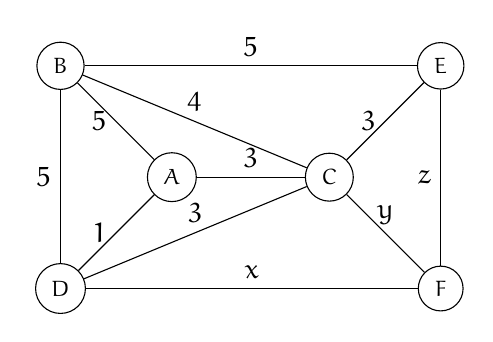
\begin{tikzpicture}[node distance = 2cm]
    \node[draw, circle] (B) {\fns\(B\)};
    \node[draw, circle, below right of = B] (A) {\fns\(A\)};
    \node[draw, circle, below left of = A] (D) {\fns\(D\)};
    \node[draw, circle, right of = A] (C) {\fns\(C\)};
    \node[draw, circle, above right of = C] (E) {\fns\(E\)};
    \node[draw, circle, below right of = C] (F) {\fns\(F\)};
    \foreach \i\j\k in {B/E/5, B/C/4, A/C/3, C/D/3, C/F/y, D/F/x} {
      \draw[] (\i) edge node[above] {\(\k\)} (\j);
    }
    \foreach \i\j\k in {A/B/5, A/D/1, C/E/3} {
      \draw[] (\i) edge node[left] {\(\k\)} (\j);
    }
    \draw[] (B) edge node[left] {\(5\)} (D);
    \draw[] (E) edge node[left] {\(z\)} (F);
  \end{tikzpicture}
\end{center}
\begin{parts}
  \part[3] Suppose \((x,y,z)=(4,1,2)\) and that we use the Kruskal's algorithm to find a minimum spanning tree of the graph. To make your answer unique and clear, please follow the rules below.
  \begin{itemize}
    \item Use \((u,v)\) to represent an undirected edge \(\{u,v\}\), where \(u<v\).
    \item Edges with same weight are sorted in alphabetical order. If two edges \(e_1=(u,v)\) and \(e_2=(w,t)\) have the same weight, \(e_1\) appears before \(e_2\) in the edge list if \((u<w)\lor\left((u=w)\land(v<t)\right)\).
  \end{itemize}
  Write down the sequence of edges added into the minimum spanning tree, and draw the tree.
  \begin{solution}
    %\vspace{2in}
    \\$(A,D)$\\
    $(C,F)$\\
    $(E,F)$\\
    $(A,C)$\\
    $(B,C)$\\

    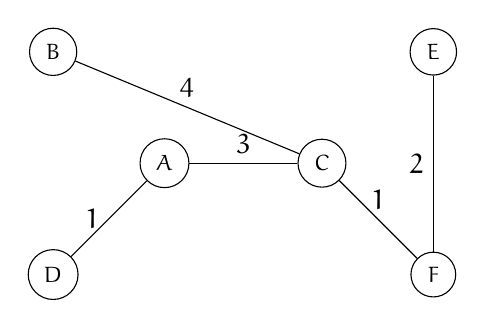
\begin{tikzpicture}[node distance = 2cm]
      \node[draw, circle] (B) {\fns\(B\)};
      \node[draw, circle, below right of = B] (A) {\fns\(A\)};
      \node[draw, circle, below left of = A] (D) {\fns\(D\)};
      \node[draw, circle, right of = A] (C) {\fns\(C\)};
      \node[draw, circle, above right of = C] (E) {\fns\(E\)};
      \node[draw, circle, below right of = C] (F) {\fns\(F\)};
      \foreach \i\j\k in {B/C/4, A/C/3, C/F/1} {
        \draw[] (\i) edge node[above] {\(\k\)} (\j);
      }
      \foreach \i\j\k in {A/D/1} {
        \draw[] (\i) edge node[left] {\(\k\)} (\j);
      }
      \draw[] (E) edge node[left] {\(2\)} (F);
    \end{tikzpicture}
    
  \end{solution}
  \part[3] If \((x,z)=(2,3)\), for what values of \(y\) is the edge \(\{C,F\}\) guaranteed to be contained in a minimum spanning tree? Give a sufficient and necessary condition and briefly justify your answer.
  \begin{solution}
    %\vspace{1in}
    \\
    the sufficient and necessary condition is $y < 3 $\\
    proof:\\
    cosider the cycle made up by the edges $(C,D),(C,F),(D,F)$
    the edge with biggest weight must not be in the MST, so we have to make sure $y$ is not the biggest weight in the cycle.
    and since $weight(C,D)=3,wight(D,F)=x=2$, so $y < 3$\\
    similarly, cosider the cycle made up by the edges $(C,E),(C,F),(E,F)$
    the edge with biggest weight must not be in the MST, so we have to make sure $y$ is not the biggest weight in the cycle.
    and since $weight(C,E)=3,wight(E,F)=z=2$, and $(C,F) must be in the cycle, $so $y < 3$\\
    so above all, the values of $y$ is $y < 3$.

  \end{solution}
  \part[2] If \(5\notin\{x,y,z\}\), is it possible for an edge weighted \(5\) to appear in a minimum spanning tree? Briefly justify your answer.
  \begin{solution}
    %\vspace{1in}
  \\
  It is impossible.\\
  proof:\\
  we can make the graph into two partitions.\\
  one set is \{A,B,C,D,E\}, and the other one is \{F\}\\
  for the first set, there exist an unique MST combined with edges \\$(A,C),(A,D),(B,C),(C,E)$
  and there weights are $1,3,4,3$, so the MST for the first set do not include edge weighted $5$.\\
  since the second set only include one vertex, so we do not need to consier its MST.\\
  to connected the two sets, and generate the MST of the whole graph, we need to take some edges which are connecting two sets.\\
  which means we will take the some of the weights in \{x,y,z\}.\\
  and since \(5 \notin \{x,y,z\}\), so the wight(s) we will take $\neq 5$\\
  so above all, it is impossible to have an edge weighted $5$ in the MST.

  \end{solution}
\end{parts}

\titledquestion{Algebraic Geometry}
Liu Big God, who loves pure math, has bought \(n\) books on algebraic geometry, the \(i\)-th of which has price \(a_i\), \(i=1,\cdots,n\). He will give his students some books to arouse their interest in pure math. For each student, Liu Big God is going to give him/her \textbf{one or two} books with total price not exceeding \(P\).

Liu Big God is not going to keep any of these books, because he has read all of them. He wants to send all these books to students. What is the minimum number of students that can receive books?

It is guaranteed that \(0\leqslant a_i\leqslant P\) for every \(i=1,\cdots,n\). You should come up with a greedy algorithm with time complexity \(O(n\log n)\).
\begin{parts}
  \part[3] Description of your algorithm in \textbf{pseudocode} or \textbf{natural language}.
  \part[4] Proof of correctness of your algorithm.
  \part[2] Time complexity.
\end{parts}

\begin{solution}
  %\vspace{5.5in}
(a) algorithm:\\
firstly sort the price array in the decending order.\\
we can use the two pointers to get the answer. So we need to set a right pointer,
which story the right-most book that has not been given out. So the initial of the right pointer is at $n$ \\
And we use the left pointer to go through the sorted sequence from left to right.\\
If the value of the book that the left pointer pointing to plus the value of the book that the right pointer pointing to is not exceeding P,
then we will give the two books to one student, and move backward the left pointer, move forward the right point.\\
otherwise, we will just give the book that left pointer pointing to to the student, and move the 
backward the left pointer.\\
At the time the left pointer and the right pointer are pointing to the same book, we will give the book to a student and finish giving books.\\
If the right pointer is on the left of the left pointer, we will immediately stop giving books because that means all books have been given out. 

(b) correctness:\\
mark the answer we get is $A$, suppose there exist an optimal solution $O$ which can give the books to less students than $A$.\\
and we can write down the solution $A$ as a pair sequence\\$(a_1,b_1),(a_2,b_2),\cdots,(a_k,b_k)$\\where $a_i,b_i$ are the value of the books that the ith student has recived.\\
and let $a_i$ be the more expensive book. If ith student only recived one book, then $b_i=0$.\\
similarly, we can also write the solution of $O$ as\\$(a_1',b_1'),(a_2',b_2'),\cdots,(a_l',b_l')$\\they have the same explanation with $A$.\\
since we consider the $O$ is optimal, then $l \leq k$.\\
Assume the first $m-1$ pairs are the same of the 2 algorithms, which means\\
$(a_m,b_m) \neq (a_m',b_m')$\\
there are three possibilities:\\
1. $a_m = a_m' , b_m \neq b_m'$\\
2. $a_m \neq a_m' , b_m = b_m'$\\
3. $a_m \neq a_m' , b_m \neq b_m'$\\
based on our $A$'s description, $a_m$ is the most value in the rest of the books, $b_m$ is the least value in the rest of the books(if $b_m \neq =$).\\
1. according to the analize above, $b_m < b_m'$, so we can just let $b_m'$ change to $b_m$, the sequence is still legal, then $(a_1,b_1),(a_2,b_2),\cdots,(a_m,b_m)$ is exactly same as \\$(a_1',b_1'),(a_2',b_2'),\cdots,(a_m',b_m')$\\
2. according to the analize above, $a_m > a_m'$, so we can just let $a_m'$ change to $a_m$, the sequence is still legal, then $(a_1,b_1),(a_2,b_2),\cdots,(a_m,b_m)$ is exactly same as \\$(a_1',b_1'),(a_2',b_2'),\cdots,(a_m',b_m')$\\
3. according to the analize above, $a_m > a_m'$ and $b_m < b_m'$, so we can just let $a_m'$ change to $a_m$ and  $b_m'$ change to $b_m$, the sequence is still legal, then $(a_1,b_1),(a_2,b_2),\cdots,(a_m,b_m)$ is exactly same as $(a_1',b_1'),(a_2',b_2'),\cdots,(a_m',b_m')$\\

Also, if there exist two pairs in $O$ such as $(a_{k_1},b_{k_1}),(a_{k_2},b_{k_2})$\\
and $a_{k_1}>a_{k_2}$, but $b_{k_1}>b_{k_2}$\\
we can just swap the $b_{k_1}$ and $b_{k_2}$, since $a_{k_1}>a_{k_2}$\\
so pairs $(a_{k_1},b_{k_2}),(a_{k_2},b_{k_1})$ are still legal, and that is same as what $A$ is doing.\\

so above all, no matter which case above, the optimal $O$ is the same with the our solution $A$.\\
so the greedy solution $A$ is the optimal.

(c) time complexity:\\
the sort of the price array $a$ takes the time of $\Theta(nlogn)$\\
and during the processing of giving out the books, each book has only been visit by one pointer once, so it takes time of $\Theta(n)$\\
so the whole time complexity is $\Theta(nlogn + n) = O(nlogn)$\\
so above all, the time complexity is $O(nlogn)$
\end{solution}

\newpage

\titledquestion{} Given a set of \(n\geqslant 3\) distinct positive numbers \(S=\left\{s_1,s_2,\cdots,s_n\right\}\), we want to find a permutation \(A=\langle A_1,\cdots,A_n\rangle\) of \(S\), where \(A_i\in S\) for all \(i\in\{1,\cdots,n\}\), such that
\[f(A)=A_1^2+\sum_{i=2}^n\left(A_i-A_{i-1}\right)^2\]
is maximized.
\begin{parts}
  \part[3] Describe your algorithm that finds the permutation \(A\) for which \(f(A)\) is maximized. Use \textbf{pseudocode} or \textbf{natural language}.
  \part[4] Prove the correctness of your algorithm by showing that your choice on the value of \(A_1\) is optimal, i.e. any other choice would not lead to a better solution.
  \part[2] Time complexity. Your algorithm should be \(O(n\log n)\).
\end{parts}

\begin{solution}
  %\vspace{5.8in}
\\
(a) algorithm:\\
sort the sequence $S$ and we can get an ascending sequence $a$.\\
and since $S$'s elements are distinct, so $a_1 < a_2 < \cdots < a_n$.\\
and let $A_1 = a_n , A_2 = a_1 , A_3 = a_{n-1} , A_4 = a_2 , \cdots$\\
let $A$ be staggered put the maximum and minimum values of $a$.
in this way, we can get the maximum $f(A)$.\\
(b) proof:\\
if we swap $a_1$ with any ohter elements in the sequence $a_i (i \neq 1)$ and get a new permutation $A'$\\
if $i=2$, then $f(A) - f(A') = 2A_3(A_1 - A_2)$,
since $A_3 > 0, A_1 = a_n = max\{a_1,\cdots,a_n\}$,
so $f(A)>f(A')$\\
if $i\neq 1$ and $i\neq 2$ and $i\neq n$, then $f(A) - f(A') = 2(A_1-A_i)(A_{i-1}+A_{i+1}-A_2)$,
since $A_1=a_n=max\{a_1,\cdots,a_n\},A_2=a_1=min\{a_1,\cdots,a_n\}$,
so $A_1-A_i > 0, A_{i-1}+A_{i+1}-A_2 > 0$\\
so $f(A) > f(A')$\\
if $i=n$, then $f(A)-f(A')=(A_1-A_n)(A_1+A_n-2A_2+2A_{n-1})$,
since $A_1=a_n=max\{a_1,\cdots,a_n\},A_2=a_1=min\{a_1,\cdots,a_n\}$,
so $A_1-A_n > 0, 2A_{n-1}-2A_2 > 0$\\
so $f(A) > f(A')$\\
so above all, if the rest of the permutation is the same, swap any of the elements with $A_1$, the $f(A)$ cannot be bigger.\\
so $A_1 = a_n$ is optimal.\\

(c) time complexity:\\
to sort the sequence $S$ takes the time complexity of $\Theta(nlogn)$\\
and calculating the function $f(A)$ takes time of $\Theta(n)$ if we can regard that the numbers are small enough to compute the multiplication and addition operations in $O(1)$ time.(i.e. high precision calculation is not required)\\
so the whole time complexity is $\Theta(nlogn + n) = O(nlogn)$\\
so above all, the time complexity is $O(nlogn)$
\end{solution}

\titledquestion{Discovery}

\begin{parts}
  \part[2] Is C++ STL \lstinline{std::sort} stable or not? If not, is there any stable sort function provided by the standard library?
  \begin{solution}
    %%%%%%%%%%%%%%%%%%%%%%%%%%%%%%%%%%%%%%%%%%%%%%%%%
    % Replace `\vspace{0.5in}' with your answer.
    %\vspace{0.5in}
    \(C++ \ STL \ std::sort\) is not stable.

    but the \(std::stable\_sort\) is stable.

    %%%%%%%%%%%%%%%%%%%%%%%%%%%%%%%%%%%%%%%%%%%%%%%%%
  \end{solution}
  \part[0] Suppose \(A\) is an array of size \(n\). If we can find the median value of \(A\) within \(O(n)\) time, it is possible to make quick-sort \(\Theta(n\log n)\) in worst case. STFW (Search The Friendly Web) about how to find the median value in \(O(n)\) time.
  
  \begin{solution}
    %%%%%%%%%%%%%%%%%%%%%%%%%%%%%%%%%%%%%%%%%%%%%%%
    
    In the book \(Introduction oto algorithms\), and by searching the friendly internet, I found an algorithm
    called \(BFPRT\), the name is from five of its inventors.

    the algorithm is mainly decided by the following steps.
    
    \begin{itemize}
      \item divide the array into groups every five adjacent numbers
      \item for each group of numbers, we find the median of the five numbers and form a median array of the median of all groups
      \item the median of each group forms a new array
      \item recursively do the above steps
      \item finally there reamin only one number, the medium number of the whole array.
      
    \end{itemize}
    
    \(T(n) \leq  T(\frac{n}{5}) +T(\frac{7n}{10})+c \cdot n\)

    and it is proved on book and internet that \(T(n) \leq 10c \cdot n\)

    so \(T(n)=\Theta(n)\)
    
    actually, when I was learning algorithms before, I hearded that we can use stl in C++, the \(std::nth\_element(...)\) can find the 
    \(k\_th\) minimal element with in \(\Theta(n)\) time.

    the median element can be easily find by using it, so I just want to write it before scearching

    However, when I scearch the code of it clearly, I thought, and some analysis on the internet also 
    say that the time complexity of \(std::nth_element\) is \(\Theta(n)\) on average, instead of the worst case,
    the worst case might turn into \(\Theta(n^2)\)

    so it might not be the best way to find the medium number, the \(DFPRT\) algorithm can get the median in \(\Theta(n)\)
    %%%%%%%%%%%%%%%%%%%%%%%%%%%%%%%%%%%%%%%%%%%%%%%
  \end{solution}
  
  \part[0] It is known that some sorting algorithms, like quick-sort, need to swap elements. Run the following code, change the value of \(n\) and see how the output changes.
  \begin{cpp}
    #include <algorithm>
    #include <cstdlib>
    #include <iostream>
    #include <vector>

    namespace std {
      template <>
      inline void swap<int>(int &lhs, int &rhs) noexcept {
        auto tmp = lhs;
        lhs = rhs;
        rhs = tmp;
        std::cout << "swap is called.\n";
      }
    } // namespace std

    int main() {
      std::srand(19260817);
      constexpr int n = 10;
      std::vector<int> vec;
      for (auto i = 0; i != n; ++i)
        vec.push_back(std::rand());
      std::sort(vec.begin(), vec.end());
      return 0;
    }
  \end{cpp}
  From your observation, the \lstinline{swap} function is never called when \(n\leqslant\) \fillin[][2em]. What algorithm(s) does \lstinline{std::sort} use?
  \begin{solution}
    %%%%%%%%%%%%%%%%%%%%%%%%%%%%%%%%%%%%%%%%%%%%%%%
    % Replace `\vspace{0.7in}' with your answer.
    %\vspace{0.7in}
    the \lstinline{swap} function is never called when \(n\leqslant 16\) .

    the std::sort is based on the introspective sorting. It is combined with many different type
    of sorting algorithms, and it will execute different onces if it reach some different situations.

    the threshold of the std::sort is 16.

    \begin{itemize}
      \item the length of the array need to be sorted is less than or equal to the threshold
      the std::sort will execute the insertion-sort.
      
      \item the length of the array need to be sorted is more than the threshold,
        
      there is another value \(depth\_limit\), which usually set as \(2*logN\), N is the length of the array need to be sorted

      \begin{itemize}
        \item the time of the recursion is less than or equal to the \(depth\_limit\)
        
        it will execute the recursive quick-sort.

        \item the time of the recursion more than the \(depth \_ limit\)
        
        it will execute heap-sort.
      \end{itemize}

    \end{itemize}
     

    %%%%%%%%%%%%%%%%%%%%%%%%%%%%%%%%%%%%%%%%%%%%%%%
  \end{solution}
\end{parts}

\end{questions}

\end{document}